\section{Specifications}
\label{sec:specs}
\newcounter{SpecID}

\subsection{Arena}
\refstepcounter{SpecID}
\label{spec:arena}

\begin{enumerate}
  \item The arena floor is an \SI{8.4}{m} $\times$ \SI{8.4}{m} rectangle. The
        tolerance of these two dimensions is $\pm$ \SI{250}{mm}.
  \item The floor of the arena is carpeted.
  \item The layout of the arena is given in Figure~\ref{fig:arena}. This
        figure is to scale.
  \item The outer walls of the arena are at least \SI{350}{mm} high, and the
        interior surface is white plastic-coated hardboard.
  \item Each scoring zone is \SI{2}{m} $\times$ \SI{2}{m} $\pm$ \SI{100}{mm},
        resulting in a total size of \SI{6}{m} $\times$ \SI{6}{m} $\pm$ \SI{200}{mm}
        for the nine scoring zones.
  \item Scoring zones are bounded by tape around the perimeter
        and internal boundaries on the floor. The inside edge of the tape marks the outside
        edge of the scoring zone.
  \item Each wall of the arena features seven \SI{250}{mm} AprilTag markers.
        The positions of these markers is given in Figure~\ref{fig:sidewall}.
        The marker numbering is given in Figure~\ref{fig:markers}.
  \item Each robot will be assigned a corner at the start of every match to indicate its starting area.
        Corner starting areas are \SI{1000}{mm} $\pm$ \SI{50}{mm} square and will be marked by tape.
\end{enumerate}

\begin{figure}
  \centering
  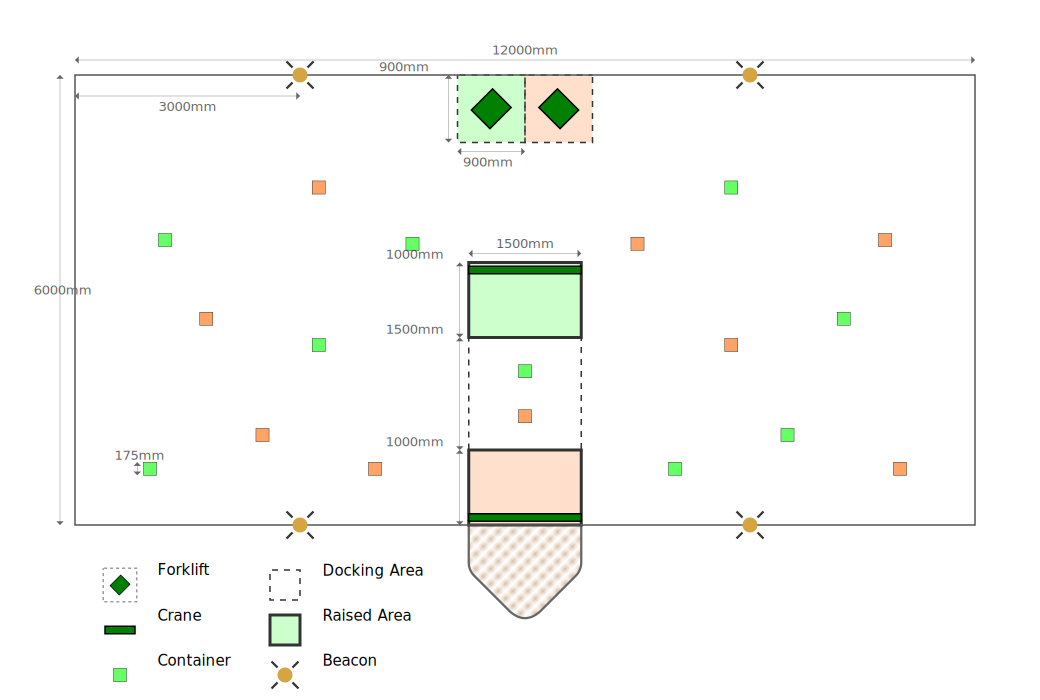
\includegraphics[scale=0.58]{fig-arena.pdf}
  \caption{Layout zones and tokens in the arena.}
  \label{fig:arena}
\end{figure}


\begin{sidewaysfigure}
  \centering
  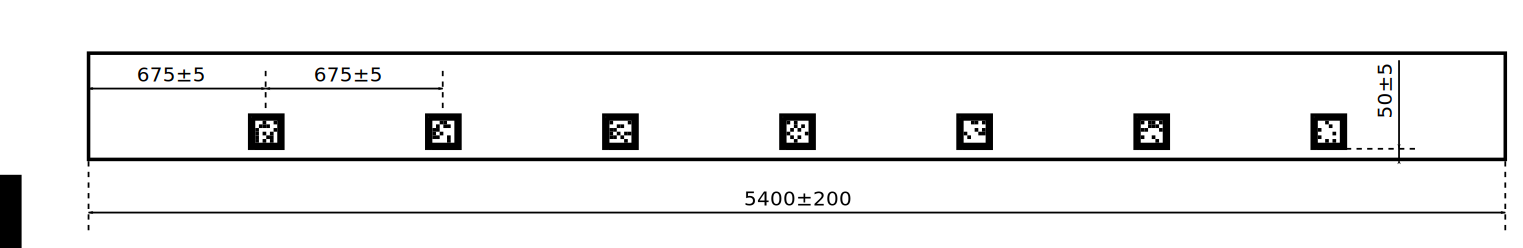
\includegraphics[scale=0.58]{fig-sidewall.pdf}
  \caption{Layout of markers along each arena wall.}
  \label{fig:sidewall}
\end{sidewaysfigure}


\begin{figure}
  \centering
  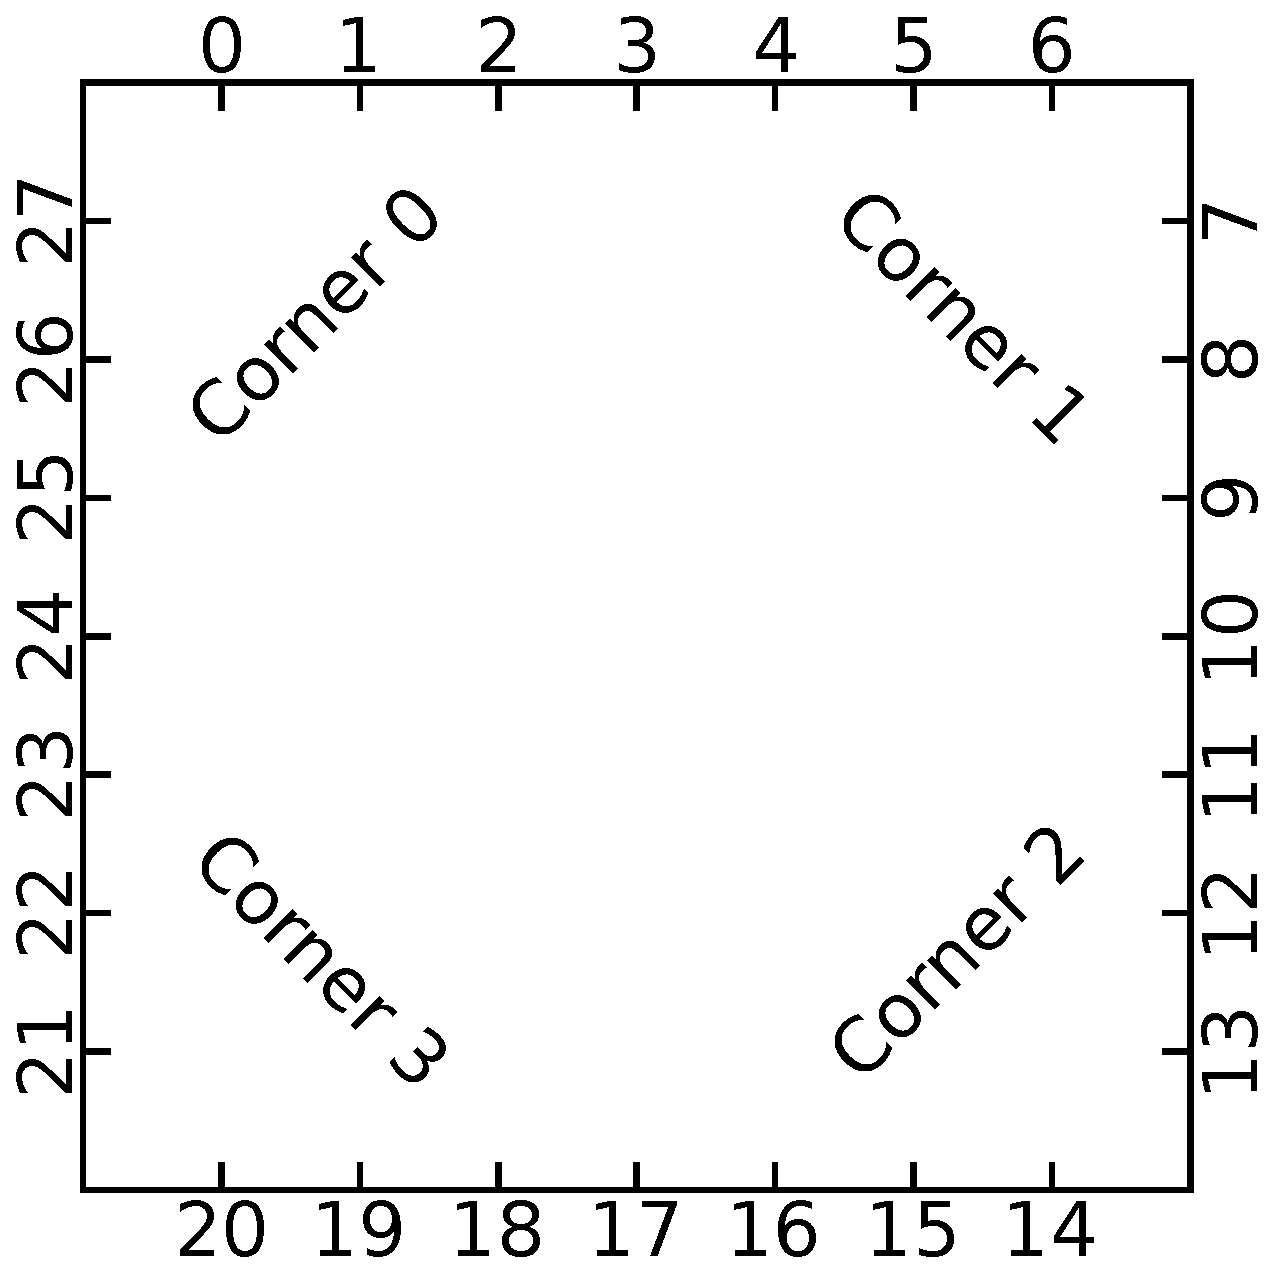
\includegraphics[scale=0.5]{fig-markers.pdf}
  \caption{Layout of markers on the arena walls.}
  \label{fig:markers}
\end{figure}

\subsection{Tokens}
\refstepcounter{SpecID}
\label{spec:tokens}

\begin{enumerate}
  \item Tokens are cuboids with side length \SI{100}{mm} $\pm$ \SI{15}{mm}.
  \item The exterior surface of a token has an AprilTag marker printed upon it. The marker is identical on all faces.
  \item All tokens belonging to the same corner will have the same marker ID.
  \item Tokens are arranged as indicated in Figure~\ref{fig:arena}.
\end{enumerate}

\begin{table}[t]
      \centering
      \begin{tabular}{lcc}
            \toprule
            \textbf{Item} & \textbf{Marker Numbers} & \textbf{Marker Size (mm)} \\
            \midrule
            Arena boundary & {} 0 -- 27 & 250 \\
            Corner 0 tokens & 28 & 80 \\
            Corner 1 tokens & 29 & 80 \\
            Corner 2 tokens & 30 & 80 \\
            Corner 3 tokens & 31 & 80 \\
            \bottomrule
      \end{tabular}
      \caption{Marker types, and the corresponding IDs and sizes.}
      \label{tab:markers}
\end{table}

\subsection{Markers}
\refstepcounter{SpecID}
\label{spec:marker}

\begin{enumerate}
  \item A `marker' is a square fiducial marker that is a member of the AprilTag 36H11 marker set.
  \item Every marker has a numeric identifier.
  \item Marker IDs are assigned according to Table~\ref{tab:markers}.
\end{enumerate}
